%!TEX root = ../Thesis.tex
\section{\glqq Was soll in die Cloud?\grqq~(An-Nam Pham)}
In Kapitel \ref{sec:IT-Infrastruktur} wurden die Vorteile für einen Umzug in die Cloud erläutert.
Da ein Teil der gesamten IT-Systemlandschaft (die zentrale Datenbank) innerhalb der Firma selbst betrieben wird, handelt es sich in diesem Fall um eine hybride Cloud, die aus der Private Cloud (zentrale Datenbank) und der Public Cloud besteht.\\
\\
Dieses Kapitel stellt unsere Empfehlung dar, was für Systeme (z.B. Module, Komponenten, etc.) in die Public Cloud installiert werden soll und was für ein Nutzen diese Systeme für das Unternehmen Stylez hat.
Die folgende Abbildung zeigt die empfohlene Implementierung der gesamten IT-Systemlandschaft. Die einzelnen Komponenten werden in den nächsten Unterkapiteln erläutert:
\begin{figure}[H]
\centering
\begin{minipage}[t]{0.8\textwidth}
\fbox{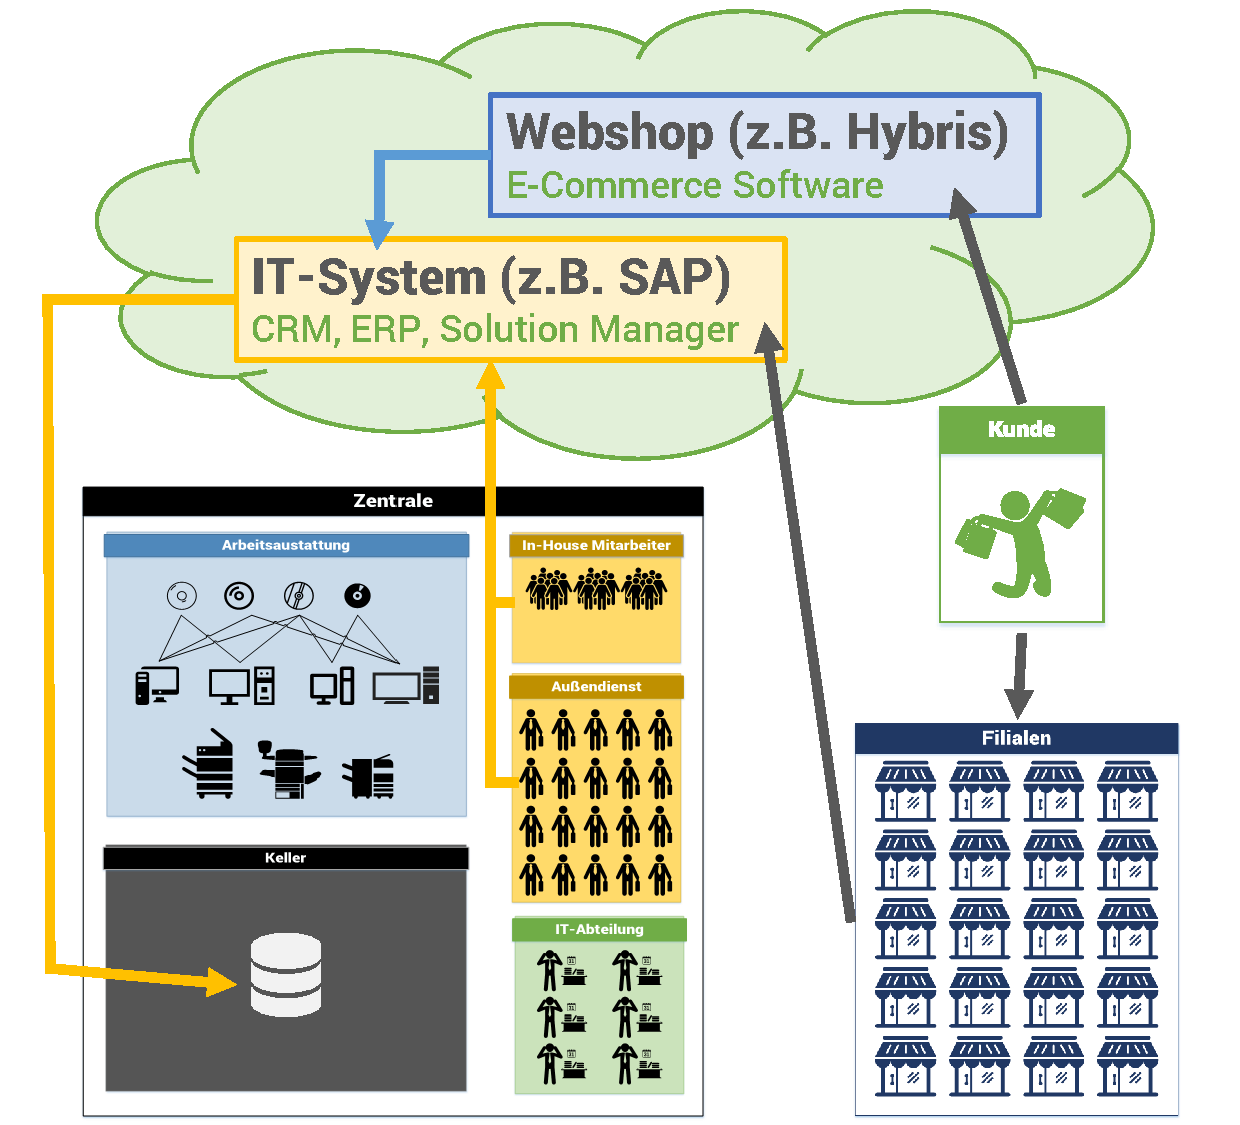
\includegraphics[width=1\textwidth]{img/Cloudinhalt.pdf}}
\caption{Empfohlene Implementierung der Hybrid Cloud} % Überschrift
\source{Eigene Darstellung} % Quelle
\label{img:Cloud_Implementierung}
\end{minipage}
\end{figure}
\subsection{SAP IT-System}
Wir empfehlen die gesamte Unternehmensstruktur von Stylez mit Hilfe von SAP im IT-System abzubilden\footnote{Berechtigungskonzept, Organisationsmanagement, Geschäftsprozesse, etc. werden in SAP ERP abgebildet, um ein optimales Business-IT-Alignment zu ermöglichen.}. Der Entscheidung für SAP bietet unter anderem folgende Vorteile\footcite{SAP_Vorteil}:
\begin{itemize}
\item Internationaler Anbieter
\item führende Technologie
\item 40 Jahre Erfahrung mit kfm. Software
\item technische Innovationskraft
\item finanzielle Stabilität
\end{itemize}
Außerdem gibt es viele SAP-Partner, die auf den Fashion-Handel spezialisiert sind. Diese haben unter anderem folgende Stärken:
\begin{itemize}
\item Kundennähe
\item Mittelstandsausrichtung und -erfahrung
\item Angebot als Generalunternehmer
\end{itemize}
Das SAP System soll aus ein ERP-System, CRM-System und einen Solution Manager bestehen.\\
\\
\underline{\textbf{SAP ERP:}}\\
Das \acrfull{ERP}
%SAP ERP (immer groß eine Überschrift mit "Der Nutzen")
%SAP CRM
%SAP Solution Manager
%SAP Rapid Deployment Solution
\subsection{Webshop}
\section{So funktioniert der Umzug in die Hybrid Cloud (An-Nam Pham)}
% \section{Stichwort: Hochverfügbarkeit}
\section{Roadmap (An-Nam Pham)}
